\section{Discovering frequent itemsets}
Ora ci occupiamo della ricerca dei \textit{frequent itemsets}. Immaginando il caso di un supermercato, andiamo a cercare gli elementi che la gente acquista insieme. 
\\
\begin{figure}[th]
    \centering
    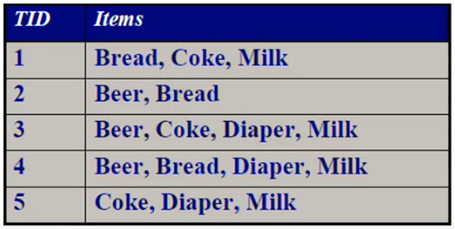
\includegraphics[scale=0.60]{FrequentItems/img/frq_itm.png}
\end{figure}
\\
E dopo aver trovato queste coppie frequenti, posso estrarre delle regole da essi:
\begin{itemize}
    \item Se qualcuno compra diaper e milk, dovrebbe comprare anche beer
    \item Discorso analogo per bread
\end{itemize}
Ma attenzione a non pensare a regole biunivoche! Sono definite in un solo verso. 

\subsection{Market-Basket model}
Il modello market-basket è utilizzato per descrivere una relazione di tipo many-many tra due tipi di oggetti. Tutti i basket hanno al loro interno degli items. Un insieme di elementi che appare \textbf{frequentemente} è un set che si ripete più volte all'interno dell'insieme dei basket. Ovvero, ci saranno n basket dove questa coppia sarà presente. Quandol è abbastanza per essere frequente? Quando n $>$ s, dove \textit{s} è un parametro chiamato \textit{soglia di supporto.}
\\
Questo parametro è importante perchè deteremina la capacità di estrapolare delle regole da un dataset. 
\begin{itemize}
    \item Se s è molto basso, ovvero ad esempio la soglia minima è che s = 1, allora riuscirò a scrivere tantissime regole, ma risulteranno completamente inutili
    \item Se s è molto alto, avviene esattamente il contrario, potrei descrivere troppo poco il dataset e impare poco sulle relazioni tra i dati
\end{itemize}
Un esempio di valore per s corrisponde all'1\% dei valori. \textbf{Attenzione!} Soglia di supporto e supporto sono diversi. Il supporto è il numero di volte che una coppia appare nel dataset, mentre la soglia è impostata per decidere se una coppia è frequente. 
\subsubsection{Principio di monotonicità}
Regola che limita il numero di frequent itemsets:
\begin{center}
    \textit{In un dataset qualunque, se sono presenti due elementi x e y frequent, avranno sicuramente una frequenza maggiore o uguale alla coppia (x,y)}
\end{center}
Ovviamente, è uguale se i due valori si ripetono sempre in tutti i basket di cui fanno parte, maggiore nel caso in cui la coppia non sia costante.

\newpage

\subsubsection{Confidence}
Un modo per misurare quanto una regola sia affidabile rispetto ad un'altra è il concetto di \textit{confidenza}.
\begin{center}
        \begin{math}
            conf(I \rightarrow j) = \frac{support(I  \cup  j)}{support(I)}
        \end{math}
\end{center}
Definita anche come la probabilità di j dato I. La utilizzo per trovare le regole che meglio descrivono i miei dati. Infatti, prendendo solo le regole che hanno confidenza più alta, sto prendendo le regole che mi forniscono più informazioni. Un'altra misura che ci interessa mantenere alta nel caso dei frequent itemset è l'\textit{interesse}:
\begin{center}
    \begin{math}
        Interest(I \rightarrow j) = |conf(I \rightarrow j) - Pr(j)|
    \end{math}
\end{center}

\subsection{Representation of the Market-Basket data}
Tipicamente, i market basket data sono salvati in un file, basket-by-basket: \{ 22, 33, 44 \} ad esempio potrebbe essere la rappresentazione di un basket. 
\\
Il numero massimo di elementi che abbiamo sono le coppie, perchè abbiamo detto che per essere frequenti un insieme di elementi deve avere delle coppie frequenti. Gli algoritmi che vedremo ora funzionano solo su coppie o terne frequenti perchè non ha senso ragionare su valori non frequenti. 
\\
\textbf{Domanda da esame: se io avessi un dataset gigantesco dove ogni riga è uno scontrino, come conto le coppie frequenti?} La cosa più banale che ci viene in mente sarebbe chiedere una lista di tutti gli elementi e con un contatore, fare il conteggio. Poi con un ciclo for per le possibili coppie, terne, ecc... Ma in un mondo big data, questo approccio è impossibile. Bisogna sfruttare il concetto di monotonicità introdotto in precedenza, e lo faccio leggendo il dataset e cercando \textbf{solo} gli elementi frequenti (diminuendo il conteggio) per poi creare delle coppie da essi e vedere quelle frequenti, e così via. Con questo approccio, ad ogni passaggio, diminuisco il numero totale di elementi da leggere. 
\\
Se avessi continuato secondo la linea d'azione originale, avrei dovuto creare (con il contatore) per ogni scontrino, un intero per vedere quante volte si ripete con tutti gli altri: per ogni scontrino avrei creato dei vettori di contatori grandi GB.
\\
Tutti gli approcci che andremo a vedere, sono caratterizzati dal numero di volte che leggo i dati.

\subsubsection{Triangular Matrix e Triplets}
Sono due tecniche che utilizziamo per fare lo storage in memoria del valore del contatore (altra operazione che ha un costo computazionale smisurato):
\begin{itemize}
    \item \textbf{Triangular Matrix:} posso considerare il vettore dei valori associando ad ogni posizione di quel valore uno specifico riferimento ad una coppia. Sui singoletti è facile, perchè l'elemento 0 è il primo elemento e quello in posto 1000 è il 1001esimo. Per le coppie è più complesso. 
    \\ 
    Come faccio con le coppie? Mi serve una funzione che mi associ ad ogni posizione, una coppia di riferimento. 
    \begin{center}
        \begin{math}
            k = (i-1)(n-\frac{i}{2} + j - i)
        \end{math}
    \end{center}
    Dove k è la posizione nel vettore, n è il numero massimo di prodotti, i e j è la coppia che voglio trovare. 
    \\
    \textit{Esempio.} Immaginiamo di avere 5 elementi, da 1 a 5. Dove sarà la coppia \{1, 4\}? 
    \begin{center}
        \begin{math}
            k = (1-1)(5-\frac{1}{2} + 4 - 1)
        \end{math}
    \end{center}
    k = 3. La coppia scelta è il terzo elemento del vettore. \textbf{Importante!} Dobbiamo considerare che i sia minore di j così da evitare i duplicati.
    \item \textbf{Triplets:} la tecnica delle triplette consiste nella creazione di una tripletta composta da i due valori numerici e il conteggio: \{1, 2, 3\} ma è svantaggioso rispetto alla matrice poichè per una coppia salva 3 interi invece di uno solo. Ha però un vantaggio enorme sulla matrice: tratta le coppie non esistenti. Nella matrice, a prescindere che una coppia si verifichi o meno, ha un posto all'interno del vettore quindi occupo la memoria con uno 0. Nel caso invece delle triplette, le coppie con conteggio nullo vengono scartate! Ed è quindi molto utile quando si usano dataset con poche coppie frequenti, altrimenti si preferisce la triangular matrix.
\end{itemize} 

\subsubsection{A-Priori Algorithm}
Creato per ridurre il numero di coppie da dover contare, fa due passaggi sui dati:
\begin{enumerate}
    \item creiamo 2 tabelle, dove la prima traduce i nomi degli items in interi. Mentre l'altra tabella è un array di conteggi. Fondamentalmente il primo step è quello utilizzato per ricercare gli elementi frequenti, candidandoli
    \item cerchiamo i singoletti non frequent e li eliminiamo. Quali sono le coppie candidate? Tutte le coppie degli elementi rimamenti, per il principio di monotonicità! 
\end{enumerate}
E alla fine valuta quali sono le coppie frequenti dopo il secondo passaggio (e non è detto che siano tutte frequent). Sicuramente efficace, ma è l'algoritmo più lento. 
\\
\begin{figure}[th]
    \centering
    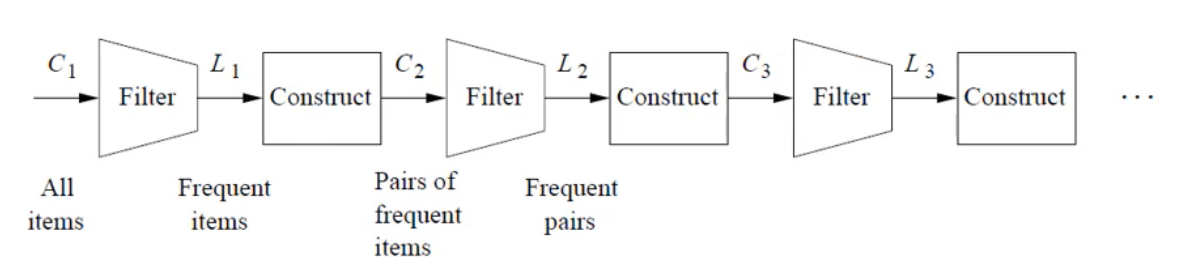
\includegraphics[scale=0.5]{FrequentItems/img/apriori.png}
\end{figure}

\subsubsection{Park, Chen, Yu Algorithm}
Simile al algoritmo precedente, sfrutta la possibilità di candidare direttamente delle coppie. Quindi nel primo passaggio avviene la generazione di coppie candidate. Utilizzando una funzione di hash non facciamo lo storage delle coppie (sarebbe troppo costoso) ma associamo ad ogni coppia un valore numerico. Quali saranno le coppie frequenti? Quelle formate da singoletti frequenti e quelle in bucket frequenti. 
\\
\textit{Esempio.} Immaginiamo di avere questa serie di elementi:
\begin{center}
    \{1,2,3\}, \{1,3,4\}, \{1,2\},  \{1,2,4\}, \{1,2,3,4\}, \{1,4\}
\end{center}
Creiamo n funzioni di hash, che chiameremo h, che contano le coppie in questo modo: h1, conta le coppie con 1, h2 quelle con 2, ecc... Il risultato è che grazie alle coppie generate dalle funzioni di hash possiamo escludere le coppie non frequenti. 

\newpage

\subsubsection{Limited Pass Algorithm}
Tecnica approssimata che non trova tutti gli item frequenti. Ragiona in un modo completamente diverso dagli altri algoritmi perchè estrae una parte degli items che possano stare in memoria e li estrae a sorte. Modifico la soglia di supporto, poichè con un dataset più piccolo, non posso usare ancora l'1\% del dataset ma prendere l'1\% del dataset più piccolo. Una volta ridotto il set, calcolo con un qualunque algoritmo visto finora. Il risultato che ottengo, impongo che sia il risultato del dataset completo, ma ovviamente lavorare solamente su un subset produrrà molti errori. Soprattutto, il problema principale saranno i falsi positivi: come posso ridurli? Faccio una seconda passata sul dataset leggendo gli elementi e verifico se quelli da me trovati sono frequenti! Elimino i non-frequent. I falsi negativi non sai di averli, e purtroppo è inutile cercare di correggerli, perchè vorrebbe dire applicare uno degli altri algoritmi...Posso pensare di ridurre i falsi negativi campionando un'altra parte del dataset e ripetendo le operazioni su di essa. Se dovessi trovare altri valori frequent che non lo erano nel primo subset, basterebbe aggiornarli. 
\\
C'è un'altra operazione, un po' meno dispendiosa: abbasso la soglia.  

\subsubsection{Toivonen's Algorithm}
Trova i risultati in queste due condizioni:
\begin{itemize}
    \item Trova tutti i risultati, senza falsi positivi o falsi negativi
    \item Non genera alcuna risposta
\end{itemize}
Come funziona? Sfrutta il concetto di \textit{negative border.} Gli itemset non frequenti formati da elementi frequenti (più corretto sarebbe dire itemset non frequenti, i cui sottoinsiemi sono frequenti). 
\\
Prendiamo solo una porzione, aggiorniamo la soglia, e calcoliamo gli elementi frequenti come visto nel Limited Pass. Andiamo a costruire il negative border e lo confrontiamo con il dataset nella sua interezza: se ci sono insiemi del negative border che sono frequent nel dataset, allora non produce risultato. Altrimenti il risultato ottenuto è corretto. 

\newpage

\subsubsection{SON Algorithm (Savasere, Omiecinski and Navathe)}
Dividiamo l'input in chunks e faccio andare l'algoritmo su ogni chunk. Ovviamente è necessario aggiornare la soglia! 
\\
Abbiamo diviso il carico computazionale tra n macchine. Ogni macchina mi darà un insieme di elementi frequent: paragoniamo il risultato con quello ottenuto dalle altre macchine. Possiamo dire che un elemento è frequent solo se supera la soglia anche nelle altre macchine (quindi se è frequent nelle altre). 
\\
\textit{Esempio.} Immaginiamo di avere due chunks:
\\
\begin{figure}[th]
    \centering
    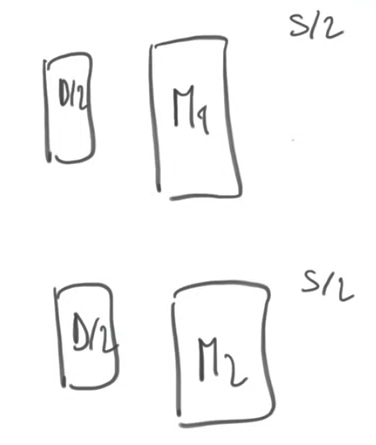
\includegraphics[scale=0.5]{FrequentItems/img/SONalgorithm.png}
\end{figure}
\\
Con le relative soglie. M1 mi estrae 4 elementi frequenti F1, F4, F7 e F9 mentre M2 mi estrae FA, F1, F4. Ora prendo l'insieme degli elementi e faccio controllare se sono frequenti in entrambe le macchine. Praticamente, passo ad M1 e M2 l'insieme di valori complessivo e conto le occorrenze in uno e nell'altro caso, se superano la soglia li posso tenere.
\\
\textbf{Approccio con MapReduce.} Il primo map mi analizza un pezzo e mi trova quelli frequenti. Mi emette una coppia chiave valore con il valore frequente e una chiave associata: per esempio. potrebbe venire una cosa di questo tipo (F1, 1), (F2, 1). Il reducer non fa assolutamente niente, butta fuori le coppie esattamente in questo modo per fare prima. Conviene piuttosto fare due cicli piuttosto che fare tutto in una volta. 
\\
Secondo step: altro mapreduce, mettiamo M1 e M2 ma questa volta con gli elementi frequenti: con il combiner possiamo contare quante occorrenze abbiamo in ogni macchina. 

\newpage

\subsection{Finding Similar Items}
Abbiamo visto come trovare gli items più frequenti, ora dobbiamo cercare di capire come trovare gli items simili. Dobbiamo trovare una misura per stabilire una similarità tra due elementi: \textbf{similarità di Jaccard}. Ossia, va analizzato un oggetto secondo un insieme di proprietà e poi è necessario guardare le proprietà che sono in comune rispetto a tutte le proprietà con cui qualifichiamo gli oggetti. Per una persona, potrebbero essere altezza, colore degli occhi, voce... Su un documento ad esempio, le parole uguali. 
\\
Perchè è utile? Per trovare documenti uguali, quindi plagiati, oppure per trovare i suggerimenti di acquisto per le persone; si vede bene la pipeline guardando la seguente immagine:
\\
\begin{figure}[th]
    \centering
    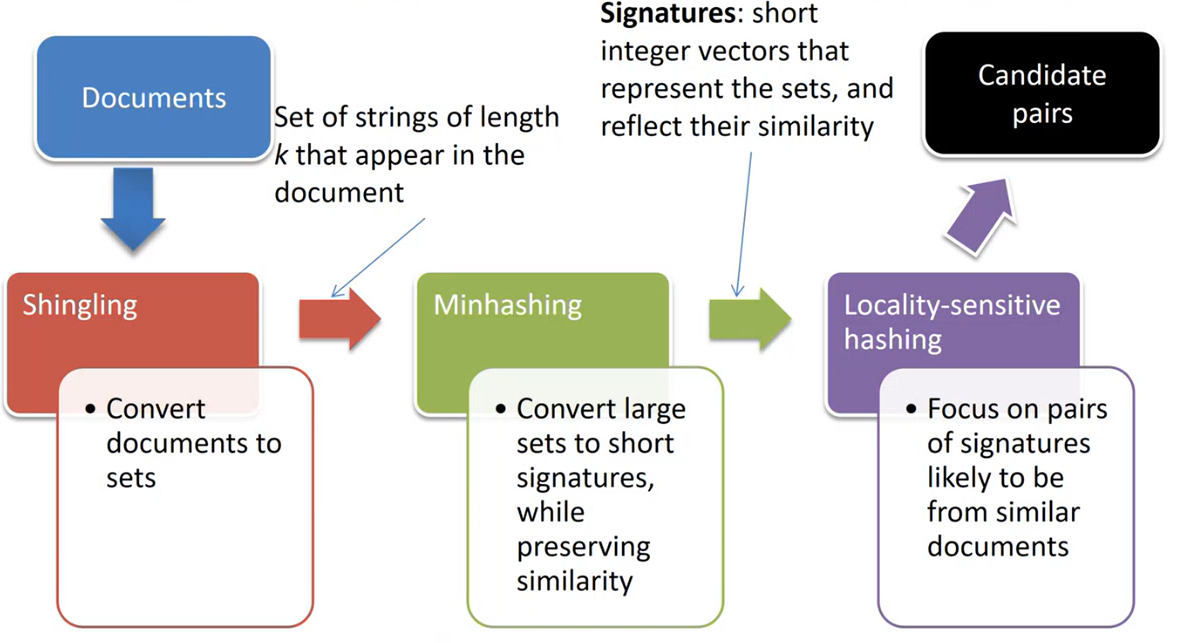
\includegraphics[scale=0.5]{FrequentItems/img/pipeline.png}
\end{figure}
\\
Tutti i passaggi verranno spiegati nello specifico qui di seguito. 

\subsubsection{Shingling}
Prima tecnica: convertiamo i documenti in insiemi. Indivuiamo una finestra di k caratteri chiamati \textit{shingle.} Vado a costruire una matrice dove sulle colonne ho sempre un milione di documenti mentre sulle righe tutte le possibili combinazioni tra caratteri. 
\\
\textit{Esempio.} Cerchiamo di capire meglio il concetto di shingle da un esempio. Frase: Oggi piove
\\
Se prendiamo k uguale a 3, otteniamo come shingle ogg, ggi, gi\_ ecc... 
\\
\textbf{Ma perchè utilizzare degli shingle?} Mi dà un ordine alle parole con questa finestra che scorre. E come scelgo k? Con un k basso, tutti i documenti risultano uguali, non faccio abbastanza distinzione se guardo in finestre unitarie di singole lettere; se k è troppo alto, ottengo al contrario una ricerca troppo pignola dove trovo solo documenti esattamente uguali (considero interi discorsi in una finestra). 
\\
\textbf{Quante righe posso fare con k=3?} Si calcolano come i caratteri che scelgo, elevati alla k: $(caratteri)^k$ e devo fare attenzione perchè per k troppo elevati, non staranno mai in memoria. 

DISCORSO MATRICCICICICIC_

\newpage

\subsubsection{Minhashing}
Seconda tecnica: tecnica per mantenere la similarità con una tabella ridotta. Riduce il numero di righe mettendo per ogni vettore della tabella originale una signature o firma che mantiene la similarità. 
\\
Prendiamo il documento originale: 